\section{Introduction}
\label{sec:intro}

One of the main objectives of \gls{qti} is to investigate if \gls{qc} can be 
used in the field of \gls{hep} in the \gls{nisq} era. Noisy means that, currently,
we have imperfect control over qubits. Intermediate refers to the number of qubits
our present quantum computers have. They range from 50 to a few hundred. 
In order to fully fulfill the promise of quantum computing, the challenges of
noise and scalability (millions of qubits) need to be solved. Nonetheless, we
can already use the available quantum computers and algorithms to tackle present
challenges. 

\gls{qml} is a growing research area that explores the interplay of ideas from \gls{qc} 
and \gls{ml}. This project explores the use of \glspl{qgan}~\cite{Zoufal_2019}, 
a \gls{qml} algorithm, to learn the kinematic distributions of the top squark (or stop) four-body 
decays~\cite{ph-brief-stop} in \gls{cms} data. The Feynman diagram for such process 
is represented in Figure~\ref{fig:model}. In \gls{hep} to simulate such 
distributions, \gls{mc} simulations are used in a very convoluted and computational
resources hungry process that can take up months. As we will see, the method 
presented in this project could speed up this process significantly when run on 
a quantum computer. This method could also be used for data augmentation of the 
\gls{mc} generated samples which would be helpful in the training of the 
classification algorithms in many \gls{hep} searches improving the sensitivity of
such searches.

\clearpage

\begin{figure}[!htbp]
\centering
	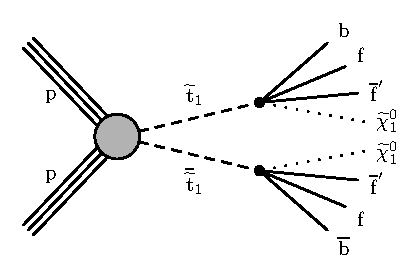
\includegraphics[width=0.70\textwidth]{figures/Figure_001.pdf}
\caption{Diagram of top squark pair production $\stp \stpb$ in $\Pp\Pp$ collisions, 
with a four-body decay of each top squark.}
\label{fig:model}
\end{figure}

This project is implemented in python~\cite{python} and will be run on a 
classical computer (my personal laptop) simulating a quantum computer with five 
qubits using pennylane~\cite{pennylane} to train and optimize the quantum 
algorithm, and cirq~\cite{cirq} for writing, manipulating, and running the 
quantum simulator.
Since \gls{qml} is a novel technique in \gls{hep}, after the present Section~\ref{sec:intro},
a brief introduction to \gls{qc} and the necessary operations needed for the 
final algorithm are presented in Section~\ref{sec:qc}. 
The main development of this project is, as well as its implementation and 
results, shown in Section~\ref{sec:demo}.
A summary and a brief discussion of futures steps after this project are 
reserved to Section~\ref{sec:sum}.